\documentclass[a4paper]{article}

\usepackage[english]{babel}
\usepackage[utf8]{inputenc}
\usepackage{amsmath}
\usepackage{graphicx}
\usepackage[colorinlistoftodos]{todonotes}
\usepackage{amsmath}
\usepackage{array}
\usepackage{multirow}
\usepackage{graphicx}
%\usepackage{subfigure}
\usepackage{subcaption}
\usepackage{tikz}
\usepackage{pgfplots}
\usepackage[colorinlistoftodos]{todonotes}
\usepackage[colorlinks=true, allcolors=blue]{hyperref}
\usepackage{placeins}
\usetikzlibrary{arrows}
\usetikzlibrary{intersections}
\usepgfplotslibrary{fillbetween}
\usepackage{setspace}

\DeclareGraphicsExtensions{.eps,.pdf,.png,.tikz}
\graphicspath{{figs/}}

\newcolumntype{M}[1]{>{\centering\arraybackslash}m{#1}}
\renewcommand\thefootnote{\textcolor{red}{\arabic{footnote}}}

\title{Backpropagation and Hebbian-LMS}

\author{JKP}

\date{\today}

\begin{document}
\maketitle

\section{LMS}

The least mean squares (LMS) algorithm is based on using the instantaneous squared error to estimate the gradient. The error is defined as the difference between the desired output $d_k$ and the output of the linear combiner $X_k^TW_K$:
\begin{equation}
\epsilon_k = d_k - X_k^TW_k
\end{equation}

We can obtain the estimate of the gradient:
\begin{equation}
\hat{\nabla} = \frac{\partial\epsilon_k^2}{\partial W} = 2\epsilon_k\frac{\partial\epsilon_k}{\partial W} = -2\epsilon_kX_k,
\end{equation}

which leads to the well-known update equations:
\begin{align} \nonumber
W_{k+1} &= W_k + 2\mu\epsilon_kX_k \\
\epsilon_k &= d_k - X_k^TW_k
\end{align}

\section{Backpropagation learning algorithm}


\section{Hebbian-LMS learning algorithm}

\subsection{Orignal Hebbian-LMS update equations}

The Hebbian-LMS neuron is essentially a bootstrapped Sigmoid-LMS neuron. The error is given by
\begin{equation}
\epsilon_k = \sigma(X_k^TW_k) - \gamma X_k^TW_k,
\end{equation}
where $\sigma$ is a sigmoid function. The gradient estimate assumes that the output of the neuron (the desired response) is independent of the weights, which is clearly not the case. The gradient estimate is then given by

\begin{equation}
\hat{\nabla} = \frac{\partial\epsilon_k^2}{\partial W} = 2\epsilon_k\frac{\partial\epsilon_k}{\partial W} = -2\epsilon_kX_k,
\end{equation}

This leads to the same LMS update equations, and it also results in two stable equilibrium points on the sigmoid. 

\subsection{Modified Hebbian-LMS update equations}
If we didn't make the assumption that the output of the sigmoid is independent of the weights, we would obtain the following gradient estimate

\begin{align}
\epsilon_k &= \mathrm{SGM}(X_k^TW_k) - \gamma X_k^TW_k, \\
\frac{\partial\epsilon_k^2}{\partial W_k} &= 2\epsilon_k\frac{\partial \epsilon_k}{\partial W_k} = 2\epsilon_k(\mathrm{SGM}^\prime(X_k^TW_k) - \gamma)X_k,
\end{align}
where $\mathrm{SGM}^\prime(x)$ denotes the first derivative of $\mathrm{SGM}(x)$. Therefore, the update equations should be
\begin{equation}
W_{k+1} = W_k - 2\mu\epsilon_k(\mathrm{SGM}^\prime(X_k^TW_k) - \gamma)X_k
\end{equation}
	
\begin{figure}[t!]
	\centering
	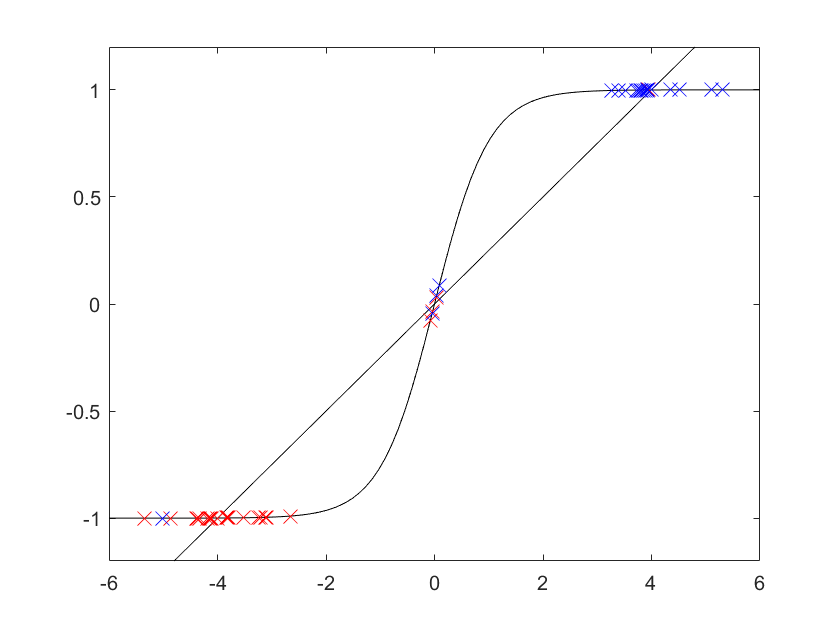
\includegraphics[scale=0.6]{figs/example-modified-hlms.png}
	\caption{Example of Hebbian-LMS clustering for the modified updated equations. Blue and red marks denote the inputs that were, respectively, positive and negative before adaptation began.}
	\label{fig:example-modified-hlms}
\end{figure}
	
With this update equation, the Hebbian-LMS neuron behaves a little differently. Clustering occurs in the two stable equilibrium points, as before, and it also occurs near the ``unstable'' equilibrium point at the origin, as shown in Fig.~\ref{fig:example-modified-hlms}. This may have an interesting effect in a Hebbian-LMS network. It would work as though the Hebbian-LMS neuron was abstaining from classifying those inputs that are clustered near the origin. However, so far the original Hebbian-LMS update equations have led to better results in terms of training error and convergence speed. 

\section{Complexity comparison between Backpropagation and Hebbian-LMS}

In a backpropagation network, training has to be realized in two passes. The forward pass, whereby the outputs of each layer are computed, and the backward pass, whereby the weights of each neuron are updated. Both of these passes have to be realized in a sequential fashion i.e., one layer at a time. In the Hebbian-LMS network, the forward pass still has to be realized sequentially, but the weights of each neuron can be updated independently. Hence, parallelization can be used to achieve extra gains in computational efficiency. This advantage is particularly relevant in today's multi-core computer architectures. 
	
\subsection{Weights update with backpropagation algorithm}

The backpropagation algorithm back-propagates the estimate of the gradient weighted by their respective weights. The backpropagation weight update procedure can be summarized in the following equations:

\begin{align} \label{eq:bp-eqs}
\delta^{(l-1)} &= (W^{(l)T}\delta^{(l)})\odot \sigma^\prime (S^{(l-1)}) \\
W^{(l)} &= W^{(l)} + 2\mu\delta^{(l)}Y^{(l-1)} \\
b^{(l)} &= b^{(l)} +  2\mu\delta^{(l)},
\end{align}
where $\odot$ denotes element-wise product of two vectors, and $\sigma^\prime(x)$ is the first derivative of the sigmoid function.
\begin{itemize}
	\item $W^{(l)}$ is a $N_w \times N_w$ matrix of the weights of the $l$th layer. $W_{ij}^{(l)}$ is the $j$th weight of the $i$th neuron. \\
	\item $b^{(l)}$ is a $N_w \times 1$ vector of the bias weights of the $l$th layer. $b_i^{(l)}$ is the bias weight of the $i$th neuron. \\
	\item $S^{(l)} = W^{(l)}Y^{(l-1)} + b^{(l)}$ is a $N_w \times 1$ vector corresponding to the output of the adders in the $l$th layer. $S_i^{(l)}$ is the output of the $i$th neuron of the $l$ layer.
	\item $Y^{(l)} = \sigma(S^{(l)})$ is a $N_w \times 1$ vector corresponding to the output of the neurons in the $l$th layer. $Y_i^{(l)}$ is the output of the $i$th neuron of the $l$ layer.
\end{itemize}

By inspecting \eqref{eq:bp-eqs}, we can conclude that the backpropagation algorithm requires the following number of floating-point operations
\begin{align} \nonumber
N_{BP, FB} &= 2(N_w - 1)N_w + N_w~\text{($\delta$ calculation)} \\ \nonumber
& + 3N_w^2~\text{(weights updates)}\\  \nonumber
& + 2N_w~\text{(bias updates)} \\
& = 5N_w^2 + N_w~\text{flops/hidden layer}
\end{align}
This only includes the hidden layers and assumes that the first layer has the same number of inputs as of all other hidden layers. Additional $N_w$ $\sigma^\prime(x)$ operations are required. 

The values of $S^{(l)}$ and $Y^{(l)}$ are calculated in the forward pass, and are assumed to be available during the backward pass. The forward pass performs $S^{(l)} = W^{(l)}Y^{(l-1)} + b^{(l)}$ and $Y^{(l)} = \sigma(S^{(l)})$. Hence,
\begin{align}
N_{BP, FF} = 2(N_w-1)N_w + N_w = 2N_w^2 - N_w ~\text{flops/hidden layer}
\end{align}
Additional $N_w$ $\sigma(x)$ operations are required. 

\subsection{Weights update with Hebbian-LMS algorithm}

For Hebbian-LMS, the number of operations required in the forward pass is the same as for backpropagation. For the weights updates, we have 
\begin{align} \label{eq:hlms-eqs}
\delta^{(l)} &= (Y^{(l)} - \gamma S^{(l)}) \\
W^{(l)} &= W^{(l)} + 2\mu\delta^{(l)}Y^{(l-1)} \\
b^{(l)} &= b^{(l)} +  2\mu\delta^{(l)}
\end{align}
For the modified Hebbian-LMS, the first equation is $\delta^{(l)} = -(Y^{(l)} - \gamma S^{(l)})\odot (\sigma^\prime(S^{(l)}) - \gamma)$.

By inspecting \eqref{eq:hlms-eqs}, we can conclude that the number of floating-point operations is
\begin{align} \nonumber
N_{HLMS} &= 2N_w ~\text{($\delta$ calculation)} \\ \nonumber
& + 3N_w^2~\text{(weights updates)}\\  \nonumber
& + 2N_w~\text{(bias updates)} \\
& = 3N_w^2 + 4N_w~\text{flops/hidden layer}
\end{align}

Table~\ref{tab:num-op} compares the number of floating-point operations required per training cycle for both backpropagation and Hebbian-LMS algorithms. The table shows how many floating-point operations are required in the calculating the outputs of the network (outputs update), and in updating the weights. For large $N_w$ or $N_l$, Hebbian-LMS uses $3/5$ of the number of operations of backprorogation.

\FloatBarrier
\begin{table} [h!]
	\caption{Number of floating-point operations required in the backpropagation and Hebbian-LMS algorithms. Additional $N_{hl}N_w~\sigma(x)$ and $N_{hl}N_w~\sigma^\prime(x)$ operations are required in the outputs update and weights update, respectively. For Hebbian-LMS the weights update operations can be parallelized so that the weights are updated simultaneously for each layer.} \label{tab:num-op}
	\centering
	\begin{tabular}{M{3.5cm}|M{3.5cm}|M{3.5cm}}
		\hline
		Algorithm & Outputs update & Weights update \\
		\hline
		Hebbian-LMS &  $N_{hl}(2N_w^2 - N_w)$ & $N_{hl}(3N_w^2 + 4N_w)$  \\
		Backpropagation & $N_{hl}(2N_w^2 - N_w)$ & $N_{hl}(5N_w^2 + N_w)$ \\
		\hline
	\end{tabular}
\end{table}
\FloatBarrier

\section{Softmax output layer}
For classification problems, it maybe be more appropriate to use the \textit{softmax} function rather than the one-out-of-many code in the output layer. With \textit{softmax}, the $i$th neuron in the output layer outputs $y_i = p(x \in K_i)$ i.e., the probability that the the input $x$ is in the $i$th cluster. Training is done to make $p(x \in K_i) = 1$ when $x \in K_i$. Hence, each output neuron is ``responsible'' for a cluster, and it'll give the probability that the input belongs to that cluster. Decisions are made by trusting the neuron that outputs the highest probability. 

The error equation for the softmax layer is given by
\begin{equation}
\epsilon_k = D - \frac{\exp{S}}{\sum\exp{S}}
\end{equation}
where $D$ is the desired response vector and $D_i = 1$ when the input vector belongs to the $i$cluster, otherwise $D_i = 0$. $S$ is the output of the linear combiner. Note that $\sum\exp{S}$ normalizes $\exp{S}$ to have a probabilistic interpretation so that $p = \frac{\exp{S}}{\sum\exp{S}}$ is a probability vector such that $p_i$ corresponds to the probability that the input vector belongs to the $i$ cluster. Moreover, note that in calculating the error, all neurons are used, whereas in the one-out-of-many code, the error is individual of each neuron.

\end{document}